% This is test report 

%\documentclass [a4paper,12pt,onecolumn] {report}

%Inclusion of required packages

%\usepackage[dvips]{graphics}
%\usepackage{color}
%\usepackage{epsfig,float}
%\usepackage{subfig}
%\usepackage{float}
%\usepackage{indentfirst}

 %\usepackage[left=2.5cm,top=2cm,right=2cm,bottom=2cm,bindingoffset=0.5cm]{geometry}
% Page layout 
%\setlength{\textwidth}{6.5in}
%\setlength{\textheight}{10in}
%\setlength{\topmargin}{0.0in}
%\setlength{\oddsidemargin}{0.0in}			% Customisable
%\setlength{\headheight}{0.0in}
%\setlength{\headsep}{0.0in}
%\setlength{\topskip}{0.0in}

% Font definition

%\fontencoding{T1}		% Font specification : Times New Roman, Bold, Normal, 18
%\fontfamily{cmr}		% Roman
%\fontseries{m}			% Medium
%\fontshape{n}			% Upright
%\fontsize{14pt}{5}		
%\selectfont			% Select the specified font

% Main report starts here

%_____________________________________________________________________________________________ 
% LATEX Template: Department of Comp/IT BTech Project Reports
% Main Report
% Sun Apr 1 20:40:00 IST 2011
% 
%_____________________________________________________________________________________________ 

\documentclass[a4paper,12pt,onecolumn]{report}

%_____________________________________________________________________________________________ 
% Inclusion of Required Packages
%_____________________________________________________________________________________________ 
\usepackage[dvips]{graphics}
\usepackage{color}
\usepackage{epsfig,float}
\usepackage[]{algorithm2e}
%_____________________________________________________________________________________________ 
% Page Layout
%_____________________________________________________________________________________________

 \usepackage[left=2.5cm,top=2cm,right=2cm,bottom=2cm,bindingoffset=0.5cm]{geometry}

%\usepackage{geometry}
%\geometry{a4paper,left=35mm,right=20mm,top=20mm,bottom=20mm}
\setlength{\textwidth}{6.5in}
\setlength{\textheight}{10in}
\setlength{\topmargin}{0.0in}
\setlength{\oddsidemargin}{0.0in}			% Customisable
\setlength{\headheight}{0.0in}
\setlength{\headsep}{0.0in}
\setlength{\topskip}{0.0in}
%_____________________________________________________________________________________________ 
% Font Definition
%_____________________________________________________________________________________________ 
\fontencoding{T1}		% Font specification : Times New Roman, Bold, Normal, 18
\fontfamily{cmr}		% Roman
\fontseries{m}			% Medium
\fontshape{n}			% Upright
\fontsize{14pt}{5}		
\linespread{1.5}		% Vertical spacing between lines
\selectfont			% Select the specified font
%_____________________________________________________________________________________________ 
% Main report starts here
%_____________________________________________________________________________________________ 


\begin{document}
% Title Page
%_____________________________________________________________________________________________ 
% Title page: Specifies a custom-made title page
%_____________________________________________________________________________________________ 
\DeclareGraphicsExtensions{.png, .ps}
\begin{titlepage}
\begin{center}
\LARGE{\bf{Timetable Management Software\\}}	% LARGE = 17.28
%\vspace{10pt}
\Large{\bf{A Project Report\\}}		% Large = 14.40
\Large{\em{Submitted by\\}}
\begin{table}[htbp]
	\begin{center}
	\begin{tabular}{ l c c l }
	\Large\bf{Aadesh G. Magare} & & & \Large\bf{111203032} \\[0.3cm] 
	\Large\bf{Sourabh G. Limbore} & & & \Large\bf{111203031} \\
	\end{tabular}
	\end{center}
	\end{table}
\Large{\em{in partial fulfillment for the award of the degree\\ \vspace{1.5pt}of\\}}
\LARGE{\bf{B.Tech Computer Engineering\\}}% Mention only appropriate degree.
%\vspace{10pt}
%names of advisors
\Large{Under the guidance of\\ }
\Large{\bf{Prof. Abhijit A. M.}\\}
\Large{College of Engineering, Pune\\}

\vspace{25pt}
%coep logo added
\begin{figure}[h]
\centering

\includegraphics[width=4cm,height=4cm]{coep_logo.jpg}
\end{figure}
\Large{\bf{DEPARTMENT OF COMPUTER ENGINEERING AND \\INFORMATION TECHNOLOGY,\\ 
COLLEGE OF ENGINEERING, PUNE-5}}
\vfill
\large{May, 2016}
\end{center}
\end{titlepage}


% Certificate Page
%_____________________________________________________________________________________________ 
% LATEX Template: Department of Comp/IT BTech Project Reports
% Certificate Page
% Sun Mar 27 10:25:35 IST 2011
% 
% Note: UK English spellings used. 
%_____________________________________________________________________________________________ 
\thispagestyle{empty}
\linespread{2}
\begin{center}			% LARGE = 18
	\Large{\bf{DEPARTMENT OF COMPUTER ENGINEERING AND\\  INFORMATION TECHNOLOGY,\\ 
	       COLLEGE OF ENGINEERING, PUNE\\}}	
\end{center}

\vspace{20pt}			% Vertical space between dept name and ``certi''

\begin{center}
	\Large{\bf{CERTIFICATE\\}}
\end{center}

\vspace{20pt}

\linespread{1.5}			% Double spacing between lines
\selectfont
\large{
Certified that this project, titled Timetable Management Software
has been successfully completed by \\ 
\begin{table}[htbp]
	\begin{center}
	\begin{tabular}{ l c c l }
	\Large\bf{Aadesh G. Magare} & & & \Large\bf{111203032} \\ [0.3cm]
	\Large\bf{Sourabh G. Limbore} & & & \Large\bf{111203031} \\
	\end{tabular}
	\end{center}
	\end{table} \\
and is approved for the partial fulfillment of the requirements for the degree of 
``B.Tech. Computer Engineering''.
}

\vspace{60pt}

\begin{center}		% Horizontal spacing used to keep the signatures in columns at the ends of
			% lines

SIGNATURE\hspace{\stretch{1}}SIGNATURE\\
\normalsize{\bf{Abhijit A. M.\hspace{\stretch{1}}Vandana Inamdar\\
Project Guide\hspace{\stretch{1}}Head}\\
Department of Computer Engineering\hspace{\stretch{1}}Department of Computer Engineering\\
and Information Technology,\hspace{\stretch{1}}and Information Technology,\\
College of Engineering Pune,\hspace{\stretch{1}}College of Engineering Pune,\\
Shivajinagar, Pune - 5.\hspace{\stretch{1}}Shivajinagar, Pune - 5.}
\end{center}



% Absract
%_____________________________________________________________________________________________ 
% LATEX Template: Department of Comp/IT BTech Project Reports
% Abstract of Report
%_____________________________________________________________________________________________ 
\newpage
%\begin{abstract}
%\addcontentsline{toc}{chapter}{Abstract}	% This makes sure abstract is included in contents.
\begin{center}
\Large \textbf{Abstract}
\end{center}
Time table generation is a time consuming problem faced by many educational institutes. It belongs to the class of combinatorial optimization problems. We have implemented a semi-automated approach for solving this constraint heavy problem for educational institutes like College of Engineering Pune (COEP). It allows the user to make time table as per his/her choice while ensuring all constraints are satisfied and there are no conflicts. There are some existing solutions for this problem which are fully automated but difficult to use. We adopted a much simpler approach for solving it. We have developed a desktop application using object oriented programming paradigm with a user friendly interface. \par
It supports quantification of constraints, importing data from text files, mapping and filtering of data. Basic features such as cut, copy, paste are available. One can merge, unmerge no of cells as per requirements. Venue utilisation statistics and global warnings are readily available. Keyboard shortcuts are available for frequently used functions. Timetable can be exported in pdf, html and ods formats. \par
The code is available on GitHub under General Public License (GPLv3). 
\\\texttt{https://github.com/Aadesh-Magare/Btech-Project-Timetable-Management}
%\end{abstract}

%_____________________________________________________________________________________________ 


%Table of content . Edit it 
\thispagestyle{empty}
\tableofcontents
%
%
% EDIT THIS AFTER CONTENTS ARE FILLED 
%
%
%\pagenumbering{roman}	% Lowercase roman numbering for prelim sections
% \listoftables
% \addcontentsline{toc}{chapter}{List of Tables}

%\listoffigures
%\addcontentsline{toc}{chapter}{List of Figures}

%\chapter*{List of Symbols}
%\addcontentsline{toc}{chapter}{List of Symbols}
%

%THIS IS ACCORDING TO TABLE OF CONTENT
\listoffigures
\addcontentsline{toc}{chapter}{List of Figures}

\newpage
\pagenumbering{arabic}

%_____________________________________________________________________________________________ 
% LATEX Template: Department of Comp/IT BTech Project Reports
% Sample Chapter
% Sun Mar 27 10:25:35 IST 2011
%
% Note: Itemization, enumeration and other things not shown. A sample figure is included.
%_____________________________________________________________________________________________ 

\chapter{Introduction}
%Th is is a section. We can cite a reference like this: \cite{INTERNET} 	
						% Citation. See references.tex for the entry.
Every academic institution needs timetable for its functioning. Almost all college functions are computerized but timetable generation is still manually done in many institutes. Timetable scheduling is very complex problem involving many constraints. Scheduling timetable manually is time and effort consuming task. The problem is to manage the timetable such that it will satisfy all the constraints. The constraints include clashes of classrooms and timeslots, working hours of particular teacher or classrooms, number of lectures for particular subject, lunch breaks for class, etc.

We have implemented a semi-automated approach for solving this constraint heavy problem for institutions like COEP. It will allow users to make timetable  in a semi-automated manner while ensuring that all the constraints are satisfied.

{\bfseries Limitations of fully automated approach:}
\begin{itemize}
\item All constraints need to be ready at beginning.
\item All data input is mandatory at beginning. 
\item No flexibility.
\item Algorithm works mechanically, cant be modified.
\item Personalization not possible.
\end{itemize}

{\bfseries Limitations of fully manual approach:}
\begin{itemize}
\item All constraints need to be checked manually.
\item Keeping track of data is very difficult.
\item Mechanical tasks need to be done manually.
\item Debugging timetable is really difficult.
\item Takes a lot of time.
\end{itemize}

%\subsection{Vorpal blade}
%And this is a subsection.
			
\section{Problem Statement}

To design and implement an application which can be used to manage the timetable of a department in an educational institute, ensuring that none of the constraints are violated and resources are used optimally while ensuring the flexibility of semi-automated approach.

%\begin{figure}[htbp]			
%\begin{center}
%\input{fig1.latex}			% Be sure to have the input file in the directory
%\caption{A simple figure: Square}	% This will appear in the list of figures
%\label{circle}
%\end{center}
%\end{figure}

%_____________________________________________________________________________________________ 

%_____________________________________________________________________________________________ 
% LATEX Template: Department of Comp/IT BTech Project Reports
% Sample Chapter
% Sun Mar 27 10:25:35 IST 2011
%
% Note: Itemization, enumeration and other things not shown. A sample figure is included.
%_____________________________________________________________________________________________ 

\chapter{Literature review}
\section{Existing Solutions}
There are some existing softwares which solve the problem of timetable scheduling. Given below is the list of some of the well known softwares.
\subsection{FET}
This is an open-source software for automatic timetable generation. FET has some features like automatic generation of timetable based on provided constraints data, exporting the generated timetable in pdf, csv, html formats. It runs on most of the systems including GNU/Linux, Windows, MacOS. FET is too complex for new users. Large amount of data is required initially to generate timetable. There's no flexibility in timetable generation.

\subsection{aSc Timetable}
aSc Timetable is shareware software for automatic timetable generation with user-friendly GUI. It supports automatic generation of timetable with manual adjustments. The main issue with aSc Timetable is, its neither freeware nor open-source. It is not available on GNU/Linux.	

\subsection{Mimosa}
Mimosa scheduling software is user-friendly and can be used for any organization since it focuses on core challenges of scheduling. It runs on most of the systems including GNU/Linux, Windows, MacOS. Mimosa is neither freeware nor open-source.

\begin{table}[h!]
\centering
\begin{tabular}{|l|c|c|c|c|}
\hline
{\bfseries Features } & {\bfseries FET} & {\bfseries aSc Timetable} & {\bfseries Mimosa}  \\
\hline
Automatic/Manual & fully automatic & both & both \\
 & semi-automatic &   &   \\
 \hline
 Platform & Windows & Windows & Windows  \\
  & GNU/Linux, Mac & Mac & GNU/Linux, Mac  \\
 \hline
Import data from files & yes & yes & yes \\ 
  \hline
Export  & html, xml, csv & html, xml, csv & html, xml, csv  \\
\hline
Open Source & yes & no & no  \\
\hline
\end{tabular}
\caption{Comparison of existing solutions}
\label{tab:template}
\end{table}

\newpage
\section{Proposed Solution}
The main aim is to simplify the process of timetable management. The software won't automatically generate timetable but help the user manage timetable. The solution considers both soft and hard constraints. Soft constraint violation generates warning whereas hard constraints can't be violated. It supports dynamic checking of constraints.
Timetable can be easily exported in popular formats like pdf, html and ods. 

\begin{table}[h!]
\centering
\begin{tabular}{|l|c|c|c|c|}
\hline
 {\bfseries Features} & {\bfseries Proposed Solution} \\
\hline
Automatic/Manual & semi-automatic\\
 \hline
 Platform  & Windows, GNU/Linux\\
 \hline
Import data from files & yes\\ 
  \hline
Export  & html, {\bfseries ods}, pdf \\
\hline
Open Source & yes \\
\hline
\end{tabular}
\caption{Proposed solution}
\label{tab:template}
\end{table}

%_____________________________________________________________________________________________ 

%_____________________________________________________________________________________________ 
% LATEX Template: Department of Comp/IT BTech Project Reports
% Sample Chapter
% Sun Mar 27 10:25:35 IST 2011
%
% Note: Itemization, enumeration and other things not shown. A sample figure is included.
%_____________________________________________________________________________________________ 

\chapter{System design criteria}
\section{Requirements}
The software is very lightweight and runs on a machine with bare minimum configuration. Following are the minimum software and hardware requirements for the program.
\subsection{Hardware requirements (Same as for Python platform)}
\begin{itemize}
\item Memory/RAM : 512MB.
\item Hard Disk Space : 1GB.
\item Processor : Intel Pentium 4 or later.
\end{itemize}

\subsection{Software requirements}
\begin{itemize}
\item Operating system: GNU/Linux or Windows
\item Python (v2.7)
\item Libraries: Wxpython, Wxwidgets
\item Python modules: pickle, ezodf, pdfkit
\end{itemize}

\section{Constraints}
Constraints are the rules that must be satisfied by the timetable. Hard constraints are the ones which can not be violated. Soft constraints can be violated but generates warnings.
\subsection{Hard constraints}
\begin{enumerate}
\item No clashes in \textit{teacher} / \textit{venue} / \textit{class} / \textit{batch} timetable.
\item Allocated hours of a subject in timetable should not exceed the no of hours allocated to it by the institute.
\end{enumerate}

\subsection{Soft constraints}
\begin{enumerate}
\item \textit{Teacher's} workload should not exceed maximum(max) \textit{teacher} workload.
\item \textit{Venue} capacity should be greater than or equal to \textit{class} capacity.
\item Compulsory lunch break for each \textit{class} / \textit{batch}.
\item Allocated hours for a \textit{subject} in timetable should not be less than no of hours allocated to it by the institute. 
\end{enumerate}

\newpage
\section{Approach of design}
\textit{Teacher, Venue and Classes} are the three classes that are central to the working of application. Every individual teacher, venue or class is an instance of one of these classes. User needs to input data i.e. list of teachers, venues, classes and subjects. This data can also be imported from external files. Given below is the format of data that should be followed.


\begin{table}[h!]
\centering
\begin{tabular}{|l|c|c|c|}

\hline
Teacher Name & Abbreviation & WeeklyMaxLoad & DailyMaxLoad\\
\hline
Abhijit A M & AM & 25 & 5\\
\hline
Satish Kumbhar & SSK & 28 & 5\\
\hline
Jibi Abraham & JA & 22 & 5\\
\hline
\end{tabular}
\caption{Teacher Table}
\label{tab:template}
\end{table}

\begin{table}[h!]
\centering
\begin{tabular}{|l|c|c|}

\hline
 Class Name & Abbreviation & Size\\
\hline
SYComp & SYC & 75\\
\hline
TYComp & TYC & 75\\
\hline 
\end{tabular}
\caption{Class Table}
\label{tab:template}
\end{table}

\begin{table}[h!]
\centering
\begin{tabular}{|l|c|c|}

\hline
Subject Name & Abbreviation & No of hours\\
\hline
DataStructure & DSA & 4\\
\hline
MathI & M1 & 4\\
\hline 
\end{tabular}
\caption{Subject Table}
\label{tab:template}
\end{table}


\begin{table}[h!]
\centering
\begin{tabular}{|l|c|c|}

\hline
 Venue Name & Abbreviation & Capacity\\
\hline
Academic Complex 201 & AC201 & 120\\
 \hline
Academic Complex 302 & AC302 & 120\\
\hline 
\end{tabular}
\caption{Class Table}
\label{tab:template}
\end{table}


% \begin{figure}[ht!]
% 	\centering
% 	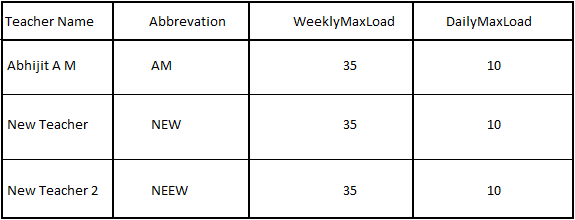
\includegraphics[width=140mm]{teacher.png}
% 	\caption{Teacher Data}
% \end{figure}

% \begin{figure}[ht!]
% 	\centering
% 	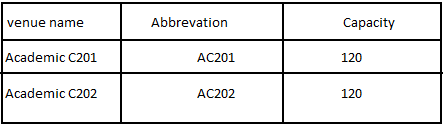
\includegraphics[width=110mm]{venue.png}
% 	\caption{Venue Data}
% \end{figure}

% \begin{figure}[ht!]
% 	\centering
% 	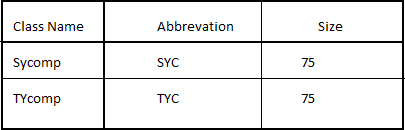
\includegraphics[width=120mm]{class.png}
% 	\caption{Class Data}
% \end{figure}

% \newpage
% \begin{figure}[ht!]
% 	\centering
% 	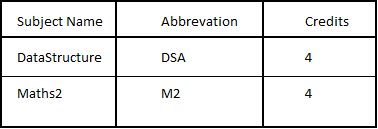
\includegraphics[width=100mm]{subject.png}
% 	\caption{Subject Data}
% \end{figure}

When user adds an entry in any of the timetable it is verified against all existing entries for violation of constraints. The change is allowed only after verification, failing which all changes are discarded. During this, constraints like teacher's work load, number of hours allocated to the subject are also checked. Venue capacity is verified for every venue-class pair. After an entry is successfully added teacher work load and subject hour count is incremented. When a hard constraint is violated all changes are discarded and an error is shown immediately. When a soft constraint is violated the warning is added to global warning section. User can view or manage global warnings any time from the menubar.



\subsection{List of Features}
\noindent
\begin{itemize}
\item Support for batches.
\item Individual teacher work load.
\item Venue-class capacity checking.
\item Venue utilization statistics.
\item Check all constraints function.
\item Pop-up box for input with dropdown suggestions.
\item Mapping and filter data in pop up box.
\item Direct typing in cell for input.
\item Mandatory lunch breaks.
\item Cut-paste / copy-paste.
\item Support for standard keyboard functions - enter, delete, backspace.
\item Import data from files.
\item Export \textit{pdf}, \textit{html} and \textit{ods}.
\item Open project with cmd argument. 
\item Save / open project.
\item Merge / unmerge selected cells.
\item Delete entry.
\item Warning list for soft constraint violation.
\item Number of hours for subject, teacher workload and venue capacity / class size changeable at runtime.

\end{itemize}
%_____________________________________________________________________________________________ 
 
 

%_____________________________________________________________________________________________ 
% LATEX Template: Department of Comp/IT BTech Project Reports
% Sample Chapter
% Sun Mar 27 10:25:35 IST 2011
%
% Note: Itemization, enumeration and other things not shown. A sample figure is included.
%_____________________________________________________________________________________________ 

\chapter{Implementation}
\section{Technologies used}
\subsection{Python} 
Python is a widely used high-level, general-purpose, interpreted, dynamic programming language. Python supports multiple programming paradigms, including object oriented, imperative and functional programming or procedural styles.
Entire application is written in python including both front end and back end. 
\subsection{wxPython}
\textit{wxPython} is a GUI toolkit for the Python programming language. It allows Python programmers to create programs with a robust, highly functional graphical user interface with ease. 

\textit{wxPython} is used for all the UI components. \textit{wx.grid}, \textit{wx.StaticText}, \textit{wx.Panel}, \textit{wx.ComboBox} are some of the important classes used in front end.
\subsection{Wxwidgets}
\textit{Wxwidgets} gives you a single, easy-to-use API for writing GUI applications on multiple platforms that still utilize the native platform's controls and utilities.
\textit{WxPython} is a python wrapper over \textit{Wxwidgets}. It makes extensive use of \textit{Wxwidgets} under the hood.
\subsection{Python modules}
\begin{itemize}
\item {\bfseries Pickle :} \textit{pickle} module implements a fundamental, but powerful algorithm for serializing and de-serializing a Python object structure.
\item {\bfseries Ezodf :} \textit{ezodf} is a Python package to create new or open existing OpenDocumentFormat files to extract, add, modify or delete document data.
\item {\bfseries Pdfkit :} \textit{wkhtmltopdf} python wrapper to convert html to pdf using the webkit rendering engine
\end{itemize}


\newpage
\section{Front-end}
GUI consist of a grid i.e. a table which is used in typical timetables. Basic constraints and header information can be provided through a window. WxPython provides classes \textit{wx.grid} class for the table UI and \textit{wx.Dialog} class for windowing purposes.

\begin{figure}[ht!]
	\centering
	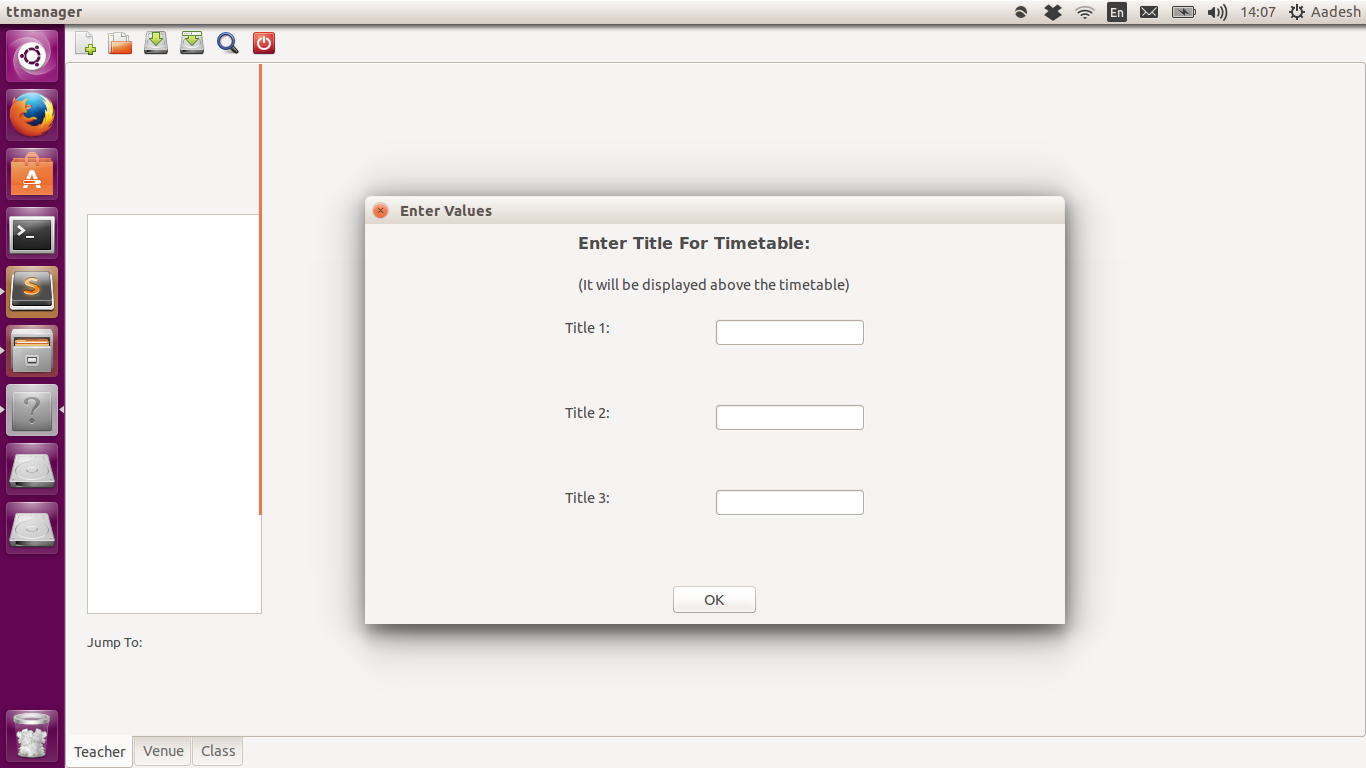
\includegraphics[width=140mm]{2.png}
	\caption{Header Information}
\end{figure}

Separate windows are available to enter teacher, venue, class and subject data. A window to enter teacher-subject, teacher-class, venue-class mappings is available. The class \textit{wx.ListCtrl} is used for all list related UI.

\newpage
An example of teacher data entry.
\begin{figure}[ht!]
	\centering
	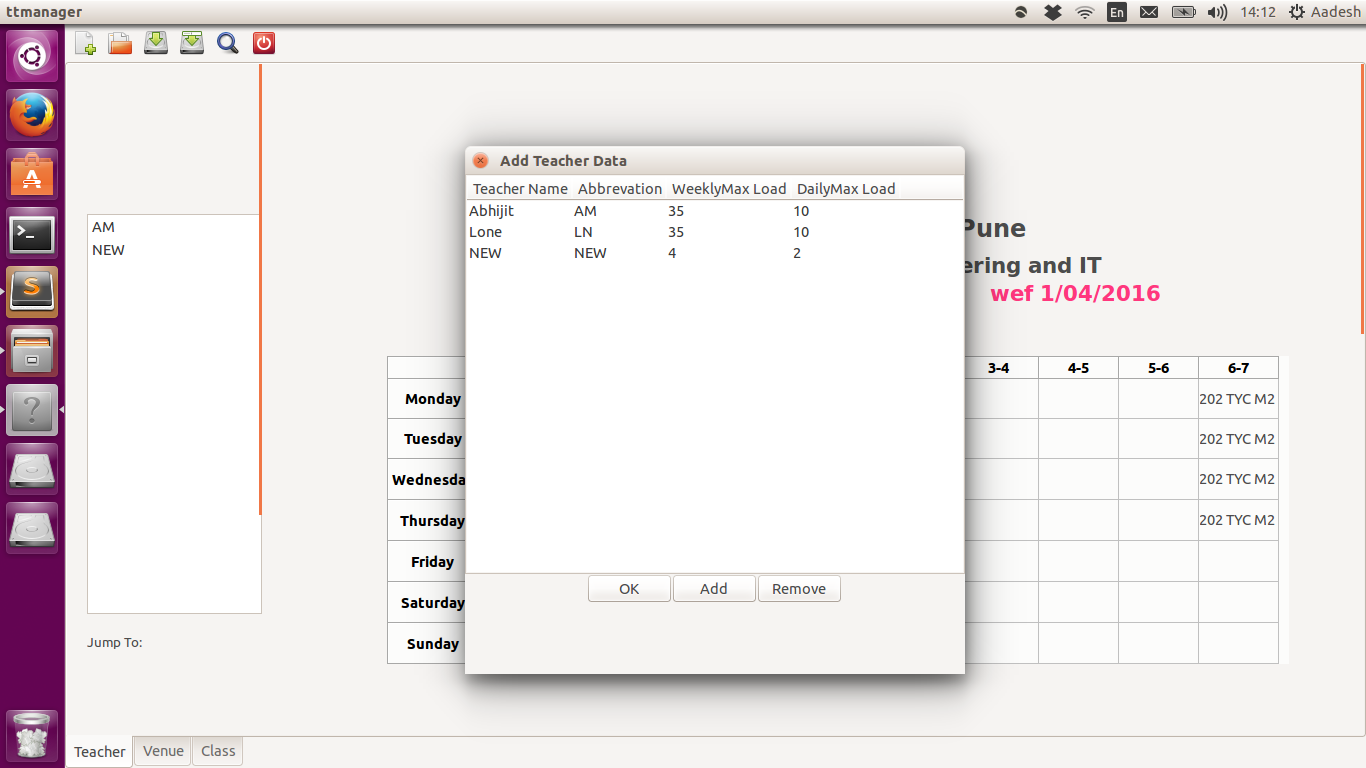
\includegraphics[width=160mm]{5.png}
	\caption{Teacher data entry}
\end{figure}

An example of venue data entry.
\begin{figure}[ht!]
	\centering
	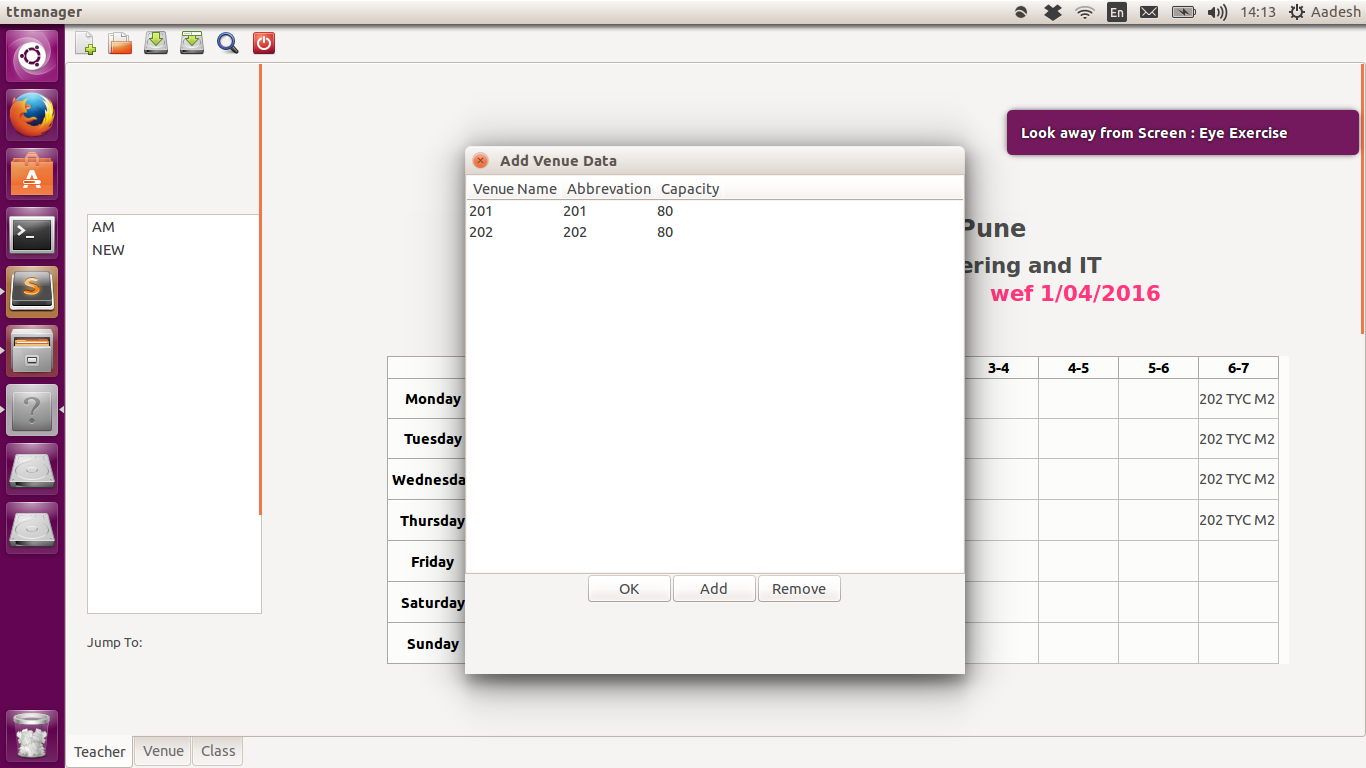
\includegraphics[width=160mm]{6.png}
	\caption{Venue data entry}
\end{figure}

\newpage
An example of venue-class mapping entry.
\begin{figure}[ht!]
	\centering
	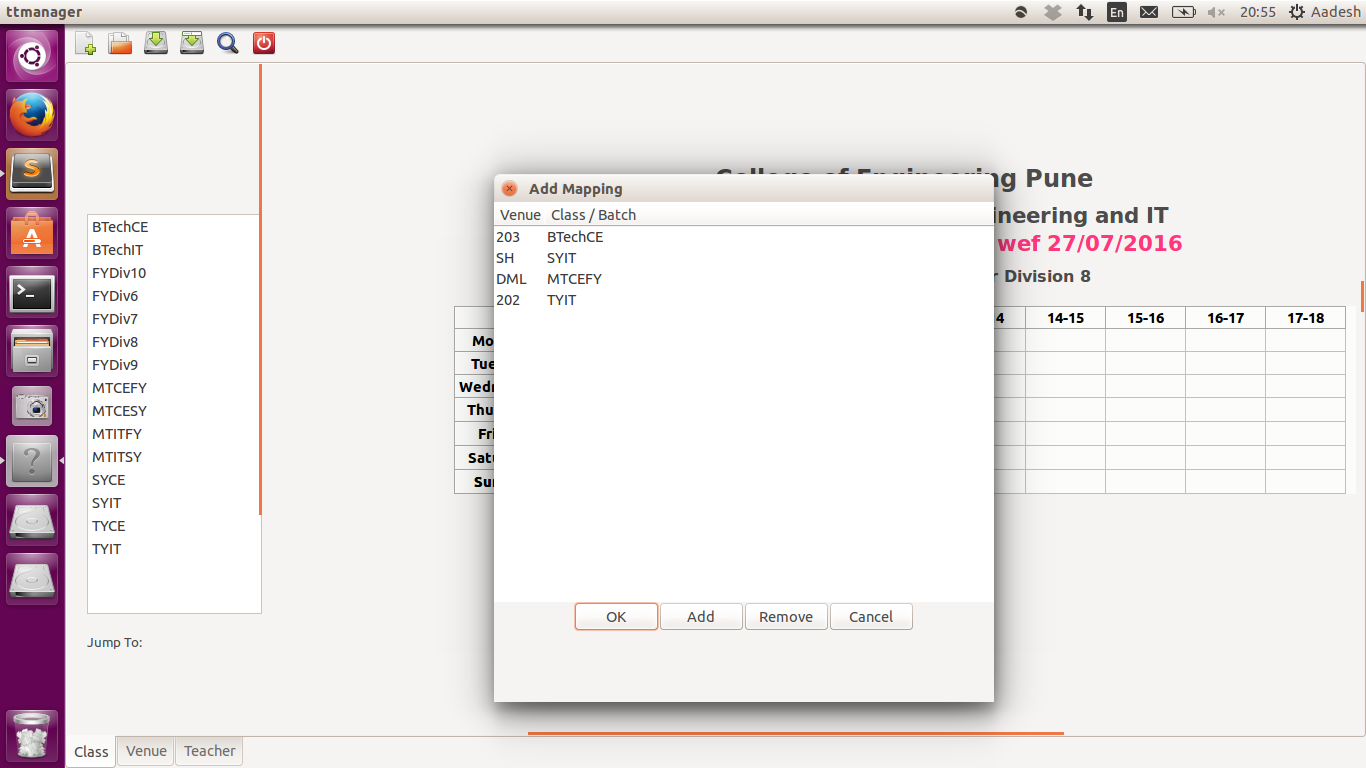
\includegraphics[width=160mm]{mapping.png}
	\caption{Venue-class mapping }
\end{figure}

An example of importing data from file.
\begin{figure}[ht!]
	\centering
	 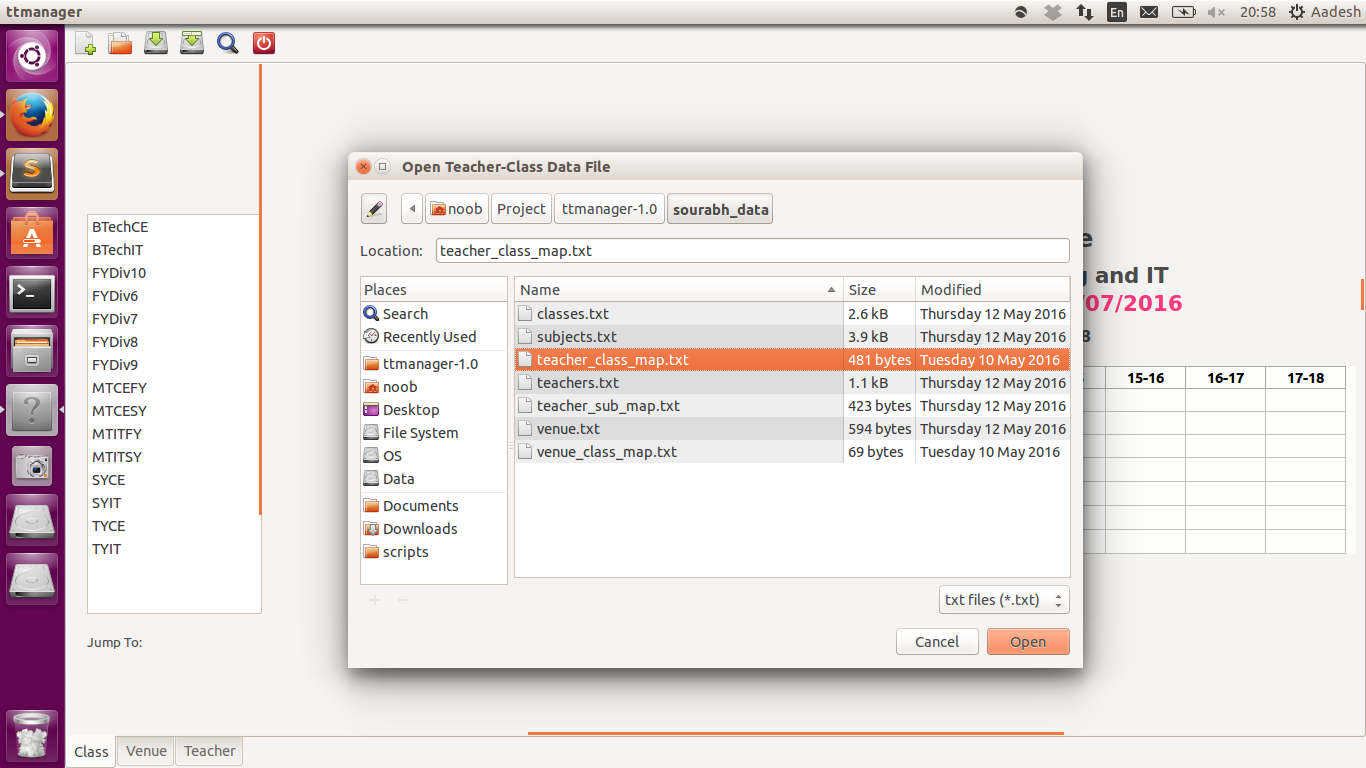
\includegraphics[width=160mm]{import_file.png}
	\caption{Importing data from file}
\end{figure}

\newpage
User can open/save partial timetable.
\begin{figure}[ht!]
	\centering
	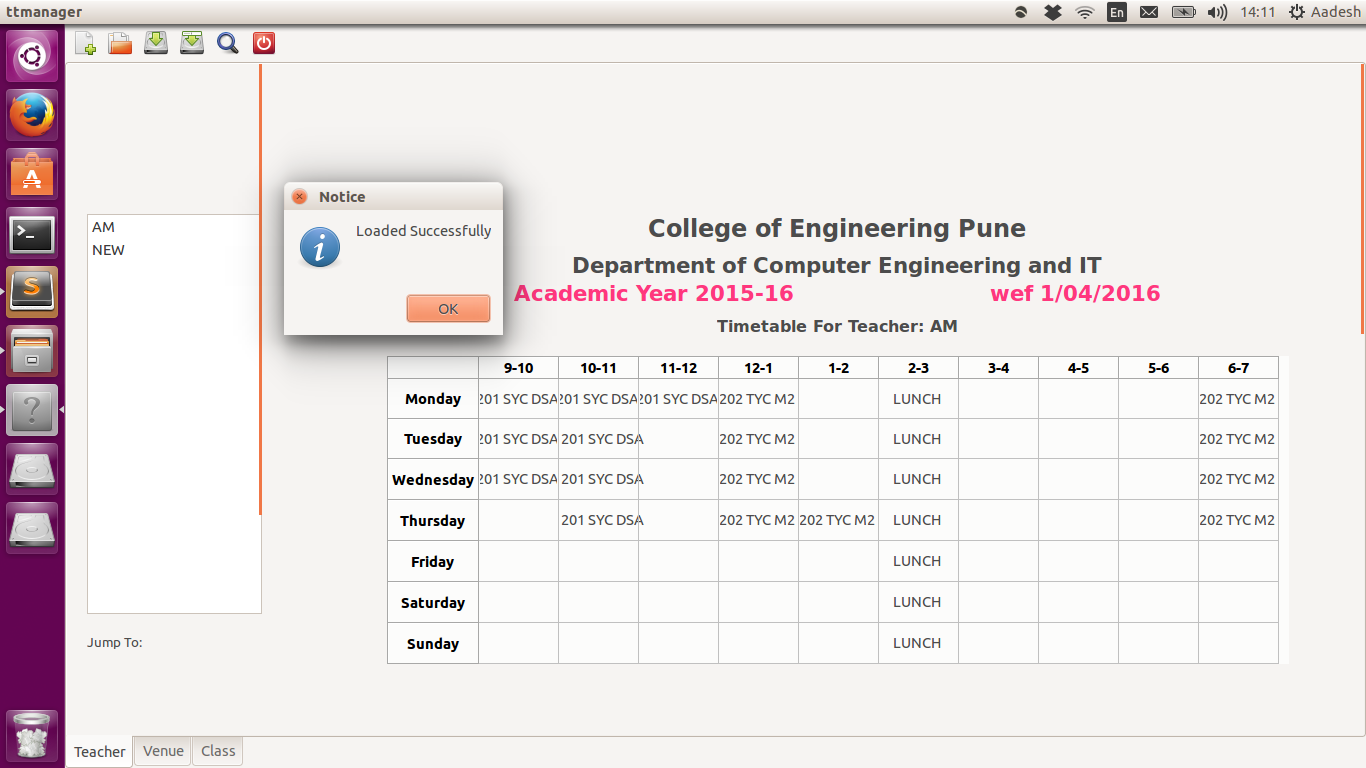
\includegraphics[width=160mm]{4.png}
	\caption{Opening of saved timetable}
\end{figure}

Pop-up boxes are used to take input from the grid. Data gathered from all these UI components is fed to back-end to initialise the timetable. Left-Panel provides easy to navigate mechanism. Double-clicking on an item scrolls to that timetable on current screen. Wxpython provides \textit{wx.lib.scrolledpanel} class for scrollable panels.

\newpage
\section{Back-end}
All data is manipulated by python scripts. \textit{Teacher, Venue, and Classes} are the User-defined class. Every teacher, venue and class involved in the timetable is an instance of these classes. These instances are stored in global lists \textit{all\_teachers}, \textit{all\_venues} and \textit{all\_classes} respectively.
These classes have methods such as can add, \textit{add\_entry}, \textit{remove\_entry} which are slightly different for each class.
% \begin{enumerate}
% \item Check teacher slot, if not available throw error and return control.
% \item If available, check teacher workload less than maximum workload.
% \item If no, show warning, goto 5.
% \item If yes, increment teacher workload, goto 5.
% \item Check venue slot, if not available remove teacher entry, throw error and return control.
% \item If available, check venue capacity less than class size.
% \item If no, show warning, goto 9.
% \item If yes, goto 9.
% \item Check class slot, if not available remove teacher and venue entry, throw error and return control.
% \item If available, entry is added to timetable and return control.
% \end{enumerate}
% {\bfseries Algorithm to insert a normal entry:}

\begin{algorithm}[H]
  \eIf{teacher slot available}{
     \eIf{teacher workload less than maximum workload}{
     		increment teacher workload\;
	   }{
	   		add warning\;
	   }
	   \eIf{venue slot available}{
     		\eIf{venue capacity less than class size}{
     			show warning\;
		   }

			\eIf{class slot available}{
		     		add entry to timetable\;
		     		return\;
			   }{
			   		remove teacher entry\;
			   		remove venue entry\;
			   		throw error and return\;
			   }  	 	
	   }{
	   		remove teacher entry\;
	   		throw error and return\;
	   }
   }{
   throw error and return\;
  }
 \caption{Algorithm to insert a entry:}
\end{algorithm}

% \newpage


{\bfseries Algorithm to add new teacher / venue / class:}

\begin{algorithm}[H]
 % \KwData{teacher/venue/class name to be added}
 % \KwResult{Object corresponding to given name}
 % initialization\;
 % \While{not at end of this document}{
 %  read current\;
  \eIf{object corresponding to name exists}{
   return it\;
   }{
   create instance of Teacher/Venue/Class depending upon type of Data\;
   push the instace into the global list of objects\;
   return the created object\;
  }
 % \caption{Algorithm to add new teacher / venue / class}
\end{algorithm}


% \begin{enumerate}
% \item Get the objects corresponding to the entry.
% \item For teacher and venue, empty that slot. For class check further.
% \item Check if entry is related to whole class or batch.
% \item If related to class, empty that slot.
% \item If related to batch, remove entry corresponding to that batch from the slot.
% \item Decrease the workload count
% \end{enumerate}
{\bfseries Algorithm to remove a entry:}

\begin{algorithm}[H]
 % \KwData{entry to be removed}
Get the objects corresponding to the entry\;
 % \While{not at end of this document}{
 %  read current\;
  \eIf{object type is teacher or venue}{
   empty that slot\;
   }{
     \eIf{entry is related to whole class}{
	   empty that slot\;
	   }{
	   remove entry corresponding to that batch from the slot\;
	   }
  }
Decrease the workload count\;
 % \caption{Algorithm to remove a entry:}
\end{algorithm}


\newpage
{\bfseries Algorithm to find venue utilization:}
% \begin{enumerate}
% \item Get all venue objects from \textit{globaldata.all\_venues}.
% \item For each object, on each working day check all lecture slots.
% \item For each non-empty entry increment the count corresponding to that venue.
% \item Find utilization relative to total available time slots.
% \end{enumerate}

\begin{algorithm}[H]
Get all venue objects from \textit{globaldata.all\_venues}\;
\While{there is next object}{
	get next object\;
	check all lecture slots on each working day\;
	for each non-empty entry increment count corresponding to that venue\;
	find utilization relative to total available time slots\;
}
 % \caption{Algorithm to find venue utilization:}
\end{algorithm}

{\bfseries Algorithm for ods export:}
% \begin{enumerate}
% \item Use the styling\_reference ods file for styling.
% \item Get save file path from user through file select box.
% \item Create three sheets named teacher, venue and class using ezodf and add to the notebook.
% \item Populate the spreadsheet for each teacher, venue and class by traversing the matrix associated with it.
% \item Use styling classes from the reference file.
% \item Save the file in user specified path.
% \end{enumerate}

\begin{algorithm}[H]
\eIf{\textit{styling\_reference.ods} file exists}{
Use the \textit{styling\_reference.ods} file for styling\;
Get save file path from user through file select box.\;
Create three sheets named teacher, venue and class using ezodf and add to the notebook.\;
Populate the spreadsheet for each teacher, venue and class by traversing the matrix associated with it.\;
Use styling classes from the reference file\;
Save the file in user specified path\;
	
}{
	show error and return\;
}
% \caption{Algorithm for ods export:}
\end{algorithm}

\newpage
{\bfseries Algorithm to verify constraints:}
% \begin{enumerate}
% \item Get all class objects from \textit{globaldata.all\_classes}.
% \item For each class check if every batch has lunch break on each working day.
% \item If not add a warning to global warnings list.
% \item For each class check if it satisfies the workload conditions or not.
% \item If not add a warning to global warnings list.
% \item For each class check if no of hours for each subject has been satisfied or not.
% \item If not add a warning to global warnings list.
% \item Get all teacher objects from \textit{globaldata.all\_teachers}.
% \item For each teacher check if every batch has lunch break on each working day.
% \item If not add a warning to global warnings list.
% \end{enumerate}


\begin{algorithm}[H]
\For{each class in \textit{globaldata.all\_classes}}{
  \eIf{every batch as lunch break on each working day}{
   }{
   add warning to global warning list\;
  }
  \eIf{workload of class is within limits}{
   }{
   add warning to global warning list\;
  }
  \eIf{no of hours for each subject satisfied}{
   }{
   add warning to global warning list\;
  }
}
\For{each teacher in \textit{globaldata.all\_teachers}}{
  \eIf{lunch break on each working day}{
   }{
   add warning to global warning list\;
  }
}
 % \caption{Algorithm to remove a entry:}
\end{algorithm}


% \newpage
Teacher and Classes class have additional methods to add / remove lunch. A lunch entry is treated differently than normal lecture entry. The Classes class has another special method valid\_lunch\_break, it is used to verify that all classes and batches have valid lunch breaks. 

\newpage
{\bfseries Algorithm to insert lunch entry:}

% \begin{enumerate}
% \item Check class (or batch) slot or teacher slot.
% \item If available entry is added to the class (or batch) or teacher.
% \item If not available, error is thrown and return control.
% \end{enumerate}

\begin{algorithm}[H]
\eIf{class slot or teacher slot available}{
	add entry to class or teacher\;
}{
	throw error\;
	return\;
}
 % \caption{Algorithm to find venue utilization:}
\end{algorithm}

A wrong entry causes Exception. In that case, its handled and its affects are undo-ed. There are 4 types of Exceptions ExistingEntry Exception, ExtraWorkLoad Exception, LimitForSubject Exception and DailyWorkLoad Exception.
\begin{enumerate}
\item {\bfseries ExistingEntry Exception :}  When the current entry clashes with existing timetable. 
\item {\bfseries ExtraWorkLoad Exception :} When the current entry exceeds the weekly workload of teacher.
\item {\bfseries LimitForSubject Exception :}  When the current entry exceeds the weekly no of lectures for a subject.
\item {\bfseries DailyWorkLoad Exception :}  When the current entry exceeds the daily workload of teacher.
\end{enumerate}

\newpage Hard constraint violation is not permitted where as soft-constraint violation causes warning which is saved in global warnings section. These global warnings are stored in file on filesystem. User can remove warnings from the file (which he/she chose to ignore). The warnings can be refreshed which causes the system to check all constraints and build the warning list again.

\textit{pickle} module is used to save the timetable on filesystem. It allows to save / open the timetable by dumping the in-memory contents on the disk. Exporting the timetable in ods, pdf and html formats is possible. Python modules \textit{ezodf} and \textit{pdfkit} are used to export the timetable. \textit{styling\_reference.ods} is used as a reference style for the ods export.

%\subsection{Vorpal blade}
%And this is a subsection.			


%_____________________________________________________________________________________________ 
 
 

%_____________________________________________________________________________________________ 
% LATEX Template: Department of Comp/IT BTech Project Reports
% Sample Chapter
% Sun Mar 27 10:25:35 IST 2011
%
% Note: Itemization, enumeration and other things not shown. A sample figure is included.
%_____________________________________________________________________________________________ 

\chapter{Conclusion}
We have implemented a software for timetable management for educational institutes. This software is helpful to manage  the timetable of a department in an educational institutes while ensuring no violation of constraints and optimal use of resources.
It provides
\begin{itemize}
\item User friendly GUI.
\item Ability to quantify constraints.
\item Import data from external files.
\item Dynamic checking of constraints.
\item Partial saving and opening of timetable.
\item Warning's window - manage warnings at one place.
\item Export timetable in ods, pdf, html format.
\end{itemize}



%\subsection{Vorpal blade}
%And this is a subsection.
			


%_____________________________________________________________________________________________ 
 
 

%_____________________________________________________________________________________________ 
% LATEX Template: Department of Comp/IT BTech Project Reports
% Sample Chapter
% Sun Mar 27 10:25:35 IST 2011
%
% Note: Itemization, enumeration and other things not shown. A sample figure is included.
%_____________________________________________________________________________________________ 

\chapter{Future Scope}
Further work can be done in following areas:
\begin{itemize}
\item Port to web-platform - to avoid installation issues and support collaborative management.
\item Automatic timetable generation. 
\item Improvement in GUI.
\item Specification of constraints.
\end{itemize}
%\subsection{Vorpal blade}
%And this is a subsection.
			


%_____________________________________________________________________________________________ 
 
 



\chapter{Diagrams}

\begin{figure}[ht!]
	\centering
	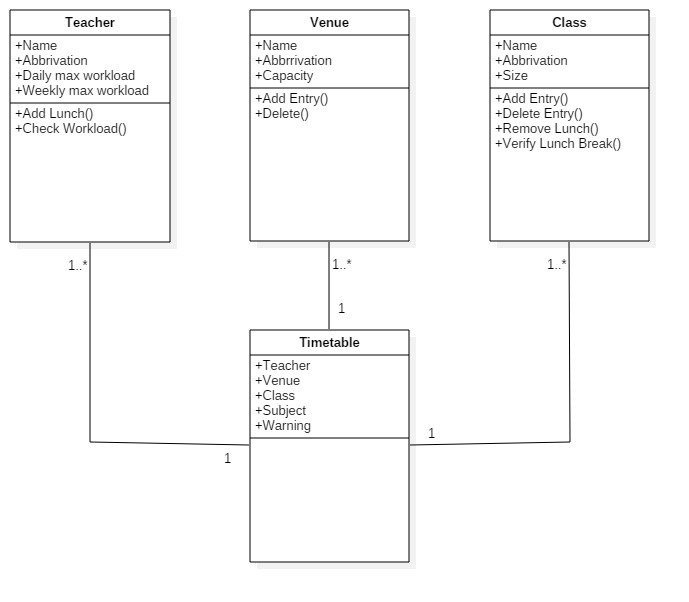
\includegraphics[height=145mm, width=130mm]{classd.jpg}
	\caption{Class Diagram}
\end{figure}

\newpage
\begin{figure}[ht!]
	\centering
	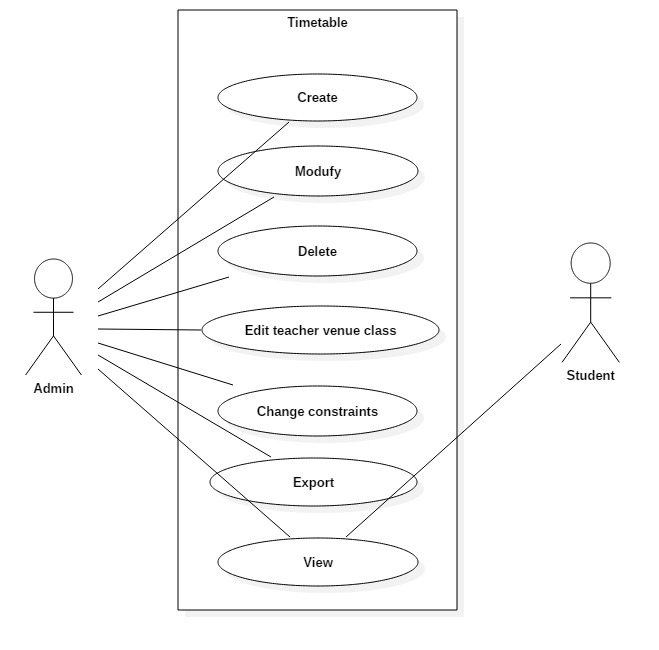
\includegraphics[height=165mm, width=130mm]{usecase.jpg}
	\caption{Use Case Diagram}
\end{figure}


\bibliography{plain}
 \medskip
    \begin{thebibliography}{9}
        \bibitem{Python }
        Python documentation,
        \\\texttt{https://docs.python.org/}   

        \bibitem{wxPython}
        wxPython,
        \\\texttt{http://www.wxpython.org/}
       
        \bibitem{wxwidgets}
        wxwidgets documentation,
        \\\texttt{https://www.wxwidgets.org/docs/tutorials/}
       
        \bibitem{ezodf}
        ezodf: Python Package,
        \\\texttt{https://pypi.python.org/pypi/ezodf}
       
        \bibitem{pickle}
        pickle: Python module,
        \\\texttt{https://docs.python.org/2/library/pickle.html}
       
        \bibitem{pdfkit}
        pdfkit: Python module,
        \\\texttt{https://pypi.python.org/pypi/pdfkit}
        
        \bibitem{GitHub}
        GitHub link of project,
        \\\texttt{https://github.com/Aadesh-Magare/Btech-Project-Timetable-Management}

    \end{thebibliography}
\end{document}\grid
\grid
